\setchapterpreamble[u]{\margintoc}
\chapter{Findings: Apps and their Artefacts}
\julian{This chapter covers \uartefacts and \iartefacts. I'm currently revising this chapter based on Arosha's feedback in late July 2022. The underlying spreadsheet of the findings is \href{https://docs.google.com/spreadsheets/d/1PcwJ6E_X6peCP1dBPADEAJXOBpnb4JY1gSGNyPSxedA/edit?usp=sharing}{Mapping content to chapters} and you should have access from your Google account if you are helping me with this thesis.}

\begin{figure*}
    \centering
    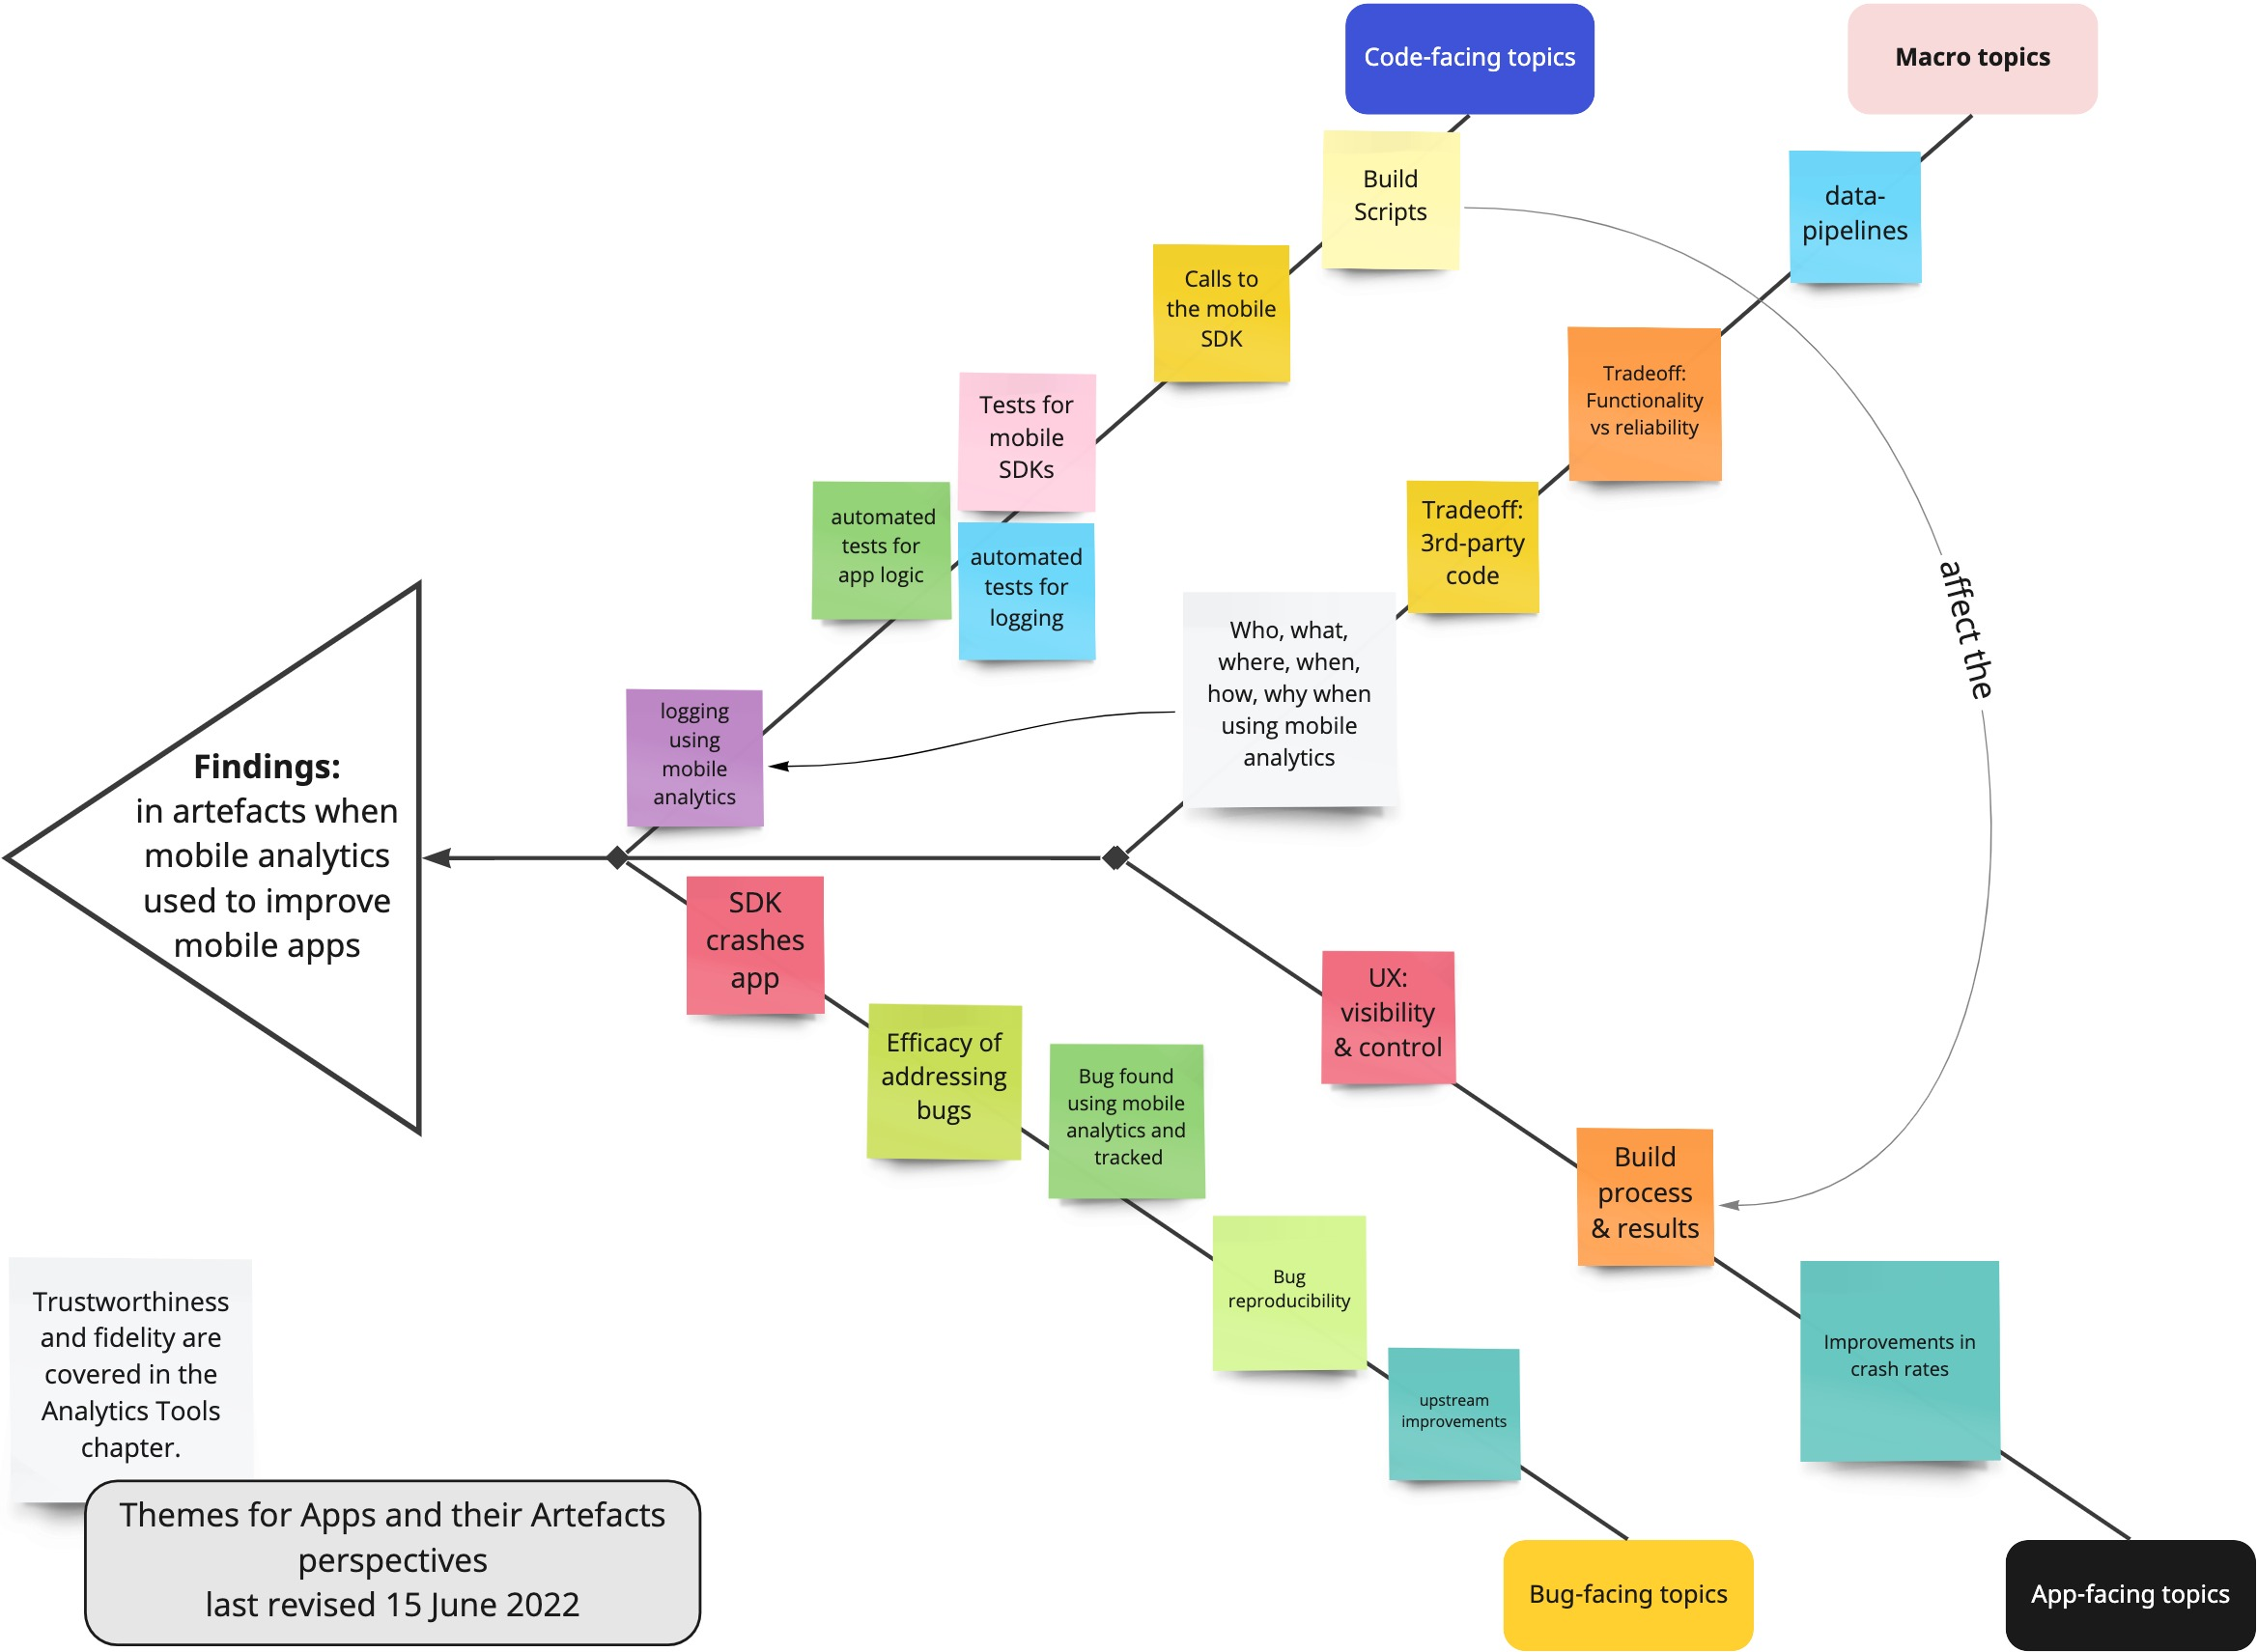
\includegraphics[width=0.8\linewidth]{images/rough-sketches/apps-and-their-artefacts-fishbone-15-jun-2022-d.jpeg}
    \caption{Apps and their artefacts fishbone diagram\\source: \href{https://miro.com/app/board/uXjVOts6mvo=/?share_link_id=402034254193}{diagram on miro.com}}
    \label{fig:apps-and-their-artefacts-fishbone}
\end{figure*}


The artefacts associated with a mobile app development project are a product (or outcome) of developers' activity as they create and maintain the app. Beyond the obvious artefacts like the source code of the app, artefacts include items stored in the bug-tracking or issue management system of the project, as well as outputs from build processes, such as test results, the release binaries and outputs from mobile analytics.

Broadly, as shown in Figure \ref{fig:apps-and-their-artefacts-fishbone}, the mobile analytics topics that are relevant to app artefacts can be organised into themes based on their relationship to the code of the app, the bugs identified in the app and the app itself. Additionally, there are a set of broader topics relating to trade offs that developers need consider when including analytics in their app artefacts and managing the data pipelines associated with analytics.

This chapter presents the findings from the case studies together with exploration of grey data and literature, relating to each of these themes. This is followed by a discussion of how mobile analytics affects the artefacts associated with a mobile app project, drawing on the broader literature on how development teams use different types of artefact.

%The artefacts are a product, an outcome, of what developers do as they create and maintain their mobile apps. They include the source code of the codebase which evolves on an ongoing basis for active projects, any bug-tracking/bug-management system, outputs from builds including test results, outputs from mobile analytics. 

%To some extent the artefacts reflect macro (big-picture) topics including ethics, scaling, data-pipelines, engineering tradeoffs, and decisions on using third-party code. Figure \ref{fig:apps-and-their-artefacts-fishbone} illustrates the topics covered in this chapter.

\section{Code-facing topics}~\label{aata-code-facing-topics}
\julian{This section needs reorganising to separate Crash and possibly Error reporting from the use of mobile analytics for other issues.}\todo{See my note here.}

The first broad category of themes relevant to the findings are associated with the artefacts of mobile app projects that are more closely connected to the code of the app. This includes 1) build scripts, 2) integration of the app with mobile analytics \Gls{sdk}s, 3) automated tests for the app, and 4) tests for mobile analytics \Gls{sdk}s. These are followed by introducing one of the ways app developers have used mobile analytics for remote logging.\todo{I suddenly realise this might fit better in the Analytics in Use chapter. I'll consider relocating it.}

\subsection{Build scripts}~\label{aata-build-scripts}
App developers use and maintain build scripts to build their apps and generally the build script combines with various build tools to customise the \gls{glossary-app-binary} (the code that's installed on app-centric mobile devices). Commonly used build variants include debug and release build targets. 
When apps include in-app mobile analytics often the build scripts are modified to specify the necessary SDK dependencies and the application's source code is modified to initialise the SDK. The documentation for Sentry's\index{Sentry} Android SDK provides a clear three step process of \textbf{Install}, \textbf{Configure}, \textbf{Verify}, so these are reproduced here~\footnote{Use permitted under their opensource license.}. Listing \ref{listing:build_gradle_for_sentry} is a typical example of how a mobile analytics dependency is added to the build file, this is Sentry's \textbf{install} step in their process.

\begin{listing}
\begin{minted}{groovy}
dependencies {
    implementation 'io.sentry:sentry-android:6.0.0'
}
\end{minted}
\caption{Example: Install Sentry \texttt{build.gradle} to an Android app's codebase\\source: \href{https://docs.sentry.io/platforms/android/}{Android Sentry Documentation}}
\label{listing:build_gradle_for_sentry}
\end{listing}

The \textbf{configuration} step requires a setting that is uniquely allocated by Sentry for this app when the developers use Sentry's online service. Listing \ref{listing:android_manifest_xml_for_sentry} shows the syntax of the configuration; the developers would need to obtain the unique dsn (data source name) to use for their app and use that value in place of the example value.

\begin{listing}
\begin{minted}{xml}
<application>
  <meta-data android:name="io.sentry.dsn"\\
  android:value="https://examplePublicKey@o0.ingest.sentry.io/0" />
</application>
\end{minted}
\caption{Example: Configure Sentry for that Android app\\source: \href{https://docs.sentry.io/platforms/android/}{Android Sentry Documentation}}
\label{listing:android_manifest_xml_for_sentry}
\end{listing}

\textbf{Verification} is not strictly part of the build scripts as it's part of the app, nonetheless it's included here since it is closely connected to the previous steps.

The code snippet in Listing \ref{listing:android_activity_to_verify_sentry_works_in_app} sends details of a caught exception to \myindex{Sentry}'s service each time the code is run. Running this code (by using the app) helps \textbf{verify} the installation and configuration steps have been completed adequately. Note: this code would generally be removed from the app once the verification has been completed successfully, developers would effectively replace it with custom code for any additional reporting not already provided automatically by the \Gls{sdk}. % https://docs.sentry.io/platforms/android/usage/  https://docs.sentry.io/platforms/android/enriching-events/breadcrumbs/  https://docs.sentry.io/platforms/android/configuration/integrations/okhttp/

During the period of this research, the SDKs have continued to evolve and tend to offer developers a greater range of information and also they tend to automated more of the underlying data collection, for example the \myindex{Sentry} 3.1.0 Android Gradle plugin automatically instruments the \myindex{OkHttp} library if it's part of the app~\sidenote{\href{https://docs.sentry.io/platforms/android/configuration/integrations/okhttp/}{docs.sentry.io/platforms/android/configuration/integrations/okhttp/}}.


\begin{listing}
\begin{minted}{kotlin}
import androidx.appcompat.app.AppCompatActivity
import android.os.Bundle
import io.sentry.Sentry

class MyActivity : AppCompatActivity() {
  override fun onCreate(savedInstanceState: Bundle?) {
    super.onCreate(savedInstanceState)
    try {
      throw Exception("This is a test.")
    } catch (e: Exception) {
      Sentry.captureException(e)
    }
  }
}
\end{minted}
\caption{Example: writing code to verify the install and configuration of the Android app\\ source: \href{https://docs.sentry.io/platforms/android/}{Android Sentry Documentation}}
\label{listing:android_activity_to_verify_sentry_works_in_app}
\end{listing}

The majority of the other SDKs used in the case studies offer equivalent installation, configuration, and verification steps and include developer-oriented documentation of these steps; note: they may use other terms to describe these steps.

\newthought{Build scripts encapsulate the build process}.  
At one extreme build scripts may fully automate multiple steps to the point of releasing a new version of an app in the app store, at the other extreme many of the steps may be manual and performed unsystematically by the development team. Of course many projects are somewhere between these two extremes, so they partly encapsulate the build process where humans have to perform the rest of the steps in the process. 

In the Catrobat case study, a mistake in a manual step of the build process meant the new release of the Pocket Code did not include the correct information and stopped the in-app crash analytics from being reported. The Crashlytics SDK on Android needed two distinct keys, an API Key and a secret key~\footnote{StackOverflow has a good example of how a build script obtains these values from the environment in \href{https://stackoverflow.com/q/46814593/340175}{stackoverflow.com/q/46814593/340175}%~\cite{scott2017_android_app_crash_noclassdeffounderror_on_samsung_lollipop_devices}
. 
The relevant documentation is no longer available, it was at \href{https://docs.fabric.io/android/fabric/settings/working-in-teams.html}{docs.fabric.io/android/fabric/settings/working-in-teams.html} according to \href{https://stackoverflow.com/a/40667490/340175}{stackoverflow.com/a/40667490/340175}}, and presumably at least one of these was either missing completely or incorrect for that build.
% https://stackoverflow.com/questions/31596792/how-to-get-test-and-production-values-for-fabric-crashlytics 
% See also https://www.instabug.com/crashlytics-alternative 
% and a nice set of examples of how to integrate various SDKs including AppSee and Crashlytics in Ruby code https://github.com/HipByte/motion-fabric 

As an aside, in Grey Data, there is an excellent example not only of configuring the API Secret Key using the runtime environment (the method used by the Catrobat project) but of an adverse side-effect of changing the build target to a newer release of Android where the app then started to crash frequently on some Samsung device models~\sidecite{scott2017_android_app_crash_noclassdeffounderror_on_samsung_lollipop_devices}. 


\subsection{Calls to the Mobile Analytics SDK}
This research found and identified several distinct uses of mobile analytics by developers. Developers could apply none, any, or even all of these uses in their app for various in-app mobile analytics SDKs.

\begin{itemize}
    \item Instantiation only: a minimal integration that calls the SDK so that it is configured and runs in the background. No other calls are made to the SDK by the app, therefore the only analytics data is whatever is collected by default by the SDK.
    \item Reporting of caught exceptions (also known as Errors and/or error reporting). 
    \item Breadcrumbs: some SDKs provide a Breadcrumbs API, for others developers can implement and use custom events to generate an instance of a breadcrumb.
    \item Reporting of additional activities: for example screen and/or network activities. This may be performed automatically by the SDK or by developers writing API calls to do so.
    \item Remote logging using a mobile analytics SDK.
\end{itemize}

\newthought{Instantiation Only}
In joint research~\sidecite{harty2021_logging_practices_with_mobile_analytics} we discovered 50 of 107 active opensource Android apps only initialised the \myindex{Firebase Analytics} \Gls{sdk}. The other 57 made additional \Gls{api} calls to the \Gls{sdk}.

\newthought{Reporting caught exceptions} 
The Commercial project, \myindex{C1}, for example, made extensive use of Microsoft App Center to record caught exceptions, in particular, while \myindex{Moonpig} used \myindex{Firebase Analytics} for similar purposes. 

\newthought{Breadcrumbs}
\myindex{Moonpig} made extensive use of Firebase Analytics to record breadcrumb information to help determine and understand what led to undesirable events.  The commercial project, \myindex{C1}, used a proprietary distributed logging API for similar purposes. \myindex{LocalHalo} \emph{might} have logged similar data using \myindex{Flurry}, their business focused mobile analytics \Gls{sdk}, they did not appear to use \myindex{Sentry} to record breadcrumbs. 

Grey literature provides code examples and screenshots of creating custom code to add and subsequently use breadcrumbs to an Android app~\sidecite{daniel2019_breadcrumbs_to_enhance_your_crashlytics_experience}. 

\newthought{Reporting of additional activities}
Both \myindex{Moonpig} and \myindex{C1} made extensive use of mobile analytics to report additional activities. For \myindex{Pocket Code} some early, exploratory code was written to experiment with recording screens and activities however this work was abandoned with the realisation that Firebase was collecting and providing demographic and other potentially sensitive information from the project team's perspective. 

Logging, network IO, and mobile analytics combined in the industrial case study where a high crash rate in a new release was caused by a flawed implementation to increase the logging of network IO through the \myindex{OkHttp} library used by the Android app. 

Various mobile analytics \Glspl{sdk} automatically record activities and network I/O, a topic for the next chapter. 

\newthought{Mobile analytics for remote logging}
Some app developers also chose to use mobile analytics for logging, for example 57 active opensource Android projects available on github.com~\sidecite{harty2021_logging_practices_with_mobile_analytics}.

Mobile Analytics \Gls{sdk}s tend to use a network connection to transmit information from the end-user's device to central servers~\sidenote{I'm not aware of any exceptions nonetheless other transfer mechanisms are possible such as using memory cards or memory sticks.}. As an aside, it should be practical to write automated tests for mobile analytics \Gls{sdk}s to check the data the \Gls{sdk} emits. Doing so is outside the scope of this research and a possible topic for future research. % I have looked at PostHog's code which is actually based heavily on a fork of Segment's opensource code so I then also looked at some of Segment's Android code. I didn't find any code that actually checks the output or the transmission aspects. Note: https://segment.com/docs/connections/sources/catalog/libraries/mobile/android/ uses Square's Tape opensource library to persist event data. This might be something to explore adding memory-card/stick transfer to.

\begin{kaobox}[frametitle=Automated tests for logging]
While logging is rarely a \emph{source} of crashes in mobile apps it's often used: 
\begin{enumerate}[label=(\alph*)]
    \item  by the platform and/or the logging SDK record the actual crash and associated stack trace~\sidenote{Crashes can be read from an Android device using developer options and the adb command \texttt{adb logcat -b crash}.}, and
    \item by the app developers to record information to help the app developers diagnose possible reasons for the crash~\sidenote{As an aside, Google developers worked with app developers to add logging to help diagnose crashes for some older Android devices \href{https://github.com/google/filament/issues/2418}{github.com/google/filament/issues/2418}.}.
\end{enumerate}

\myindex{PostHog} uses a ShadowLog in their tests of logging \\ \href{https://github.com/PostHog/posthog-android/blob/master/posthog/src/test/java/com/posthog/android/LoggerTest.java}{github.com/PostHog/posthog-android/.../LoggerTest.java}

\medskip % Vertical whitespace to allow space for the side notes without them overwriting each other.

As mentioned in \secref{section-small-experimental-android-apps} as part of this research I co-wrote various small software projects to provide automated tests of local logging by Android apps~\sidecite{android_crash_dummy, android_log_assert}\index{GitHub Projects!Android Crash Dummy}\index{GitHub Projects!Android Log Assert}; these have been released under permissive opensource licenses.

\medskip % for consistency in the layout.

These projects may provide a basis to write automated tests for remote logging using mobile analytics.
\end{kaobox}


\subsection{Use of automated tests for the app}
Automated tests can dovetail with using mobile analytics to improve the reliability of mobile apps. For example, they can be used to demonstrate the reproducibility of crashes identified through mobile analytics. In the commercial case study this is what we did for various crashes reported via Android Vitals. For one of these an equivalent example has been released as an opensource project at \href{https://github.com/julianharty/KotlinNPE}{github.com/julianharty/KotlinNPE} which tests the fix. This project is partnered by another opensource project \href{https://github.com/julianharty/AutomatedTestingWithKotlin}{github.com/julianharty/AutomatedTestingWithKotlin} as we wanted to find a way to run tests directly in a \gls{jvm} without needing the overhead of the Android runtime. When automated tests need the Android runtime the build process and the runtime environment become much more complicated and the elapsed runtime for the tests can take several orders of magnitude more time.

Use of automated tests for bug reproduction/bug fixes was patchy in all of the development teams in the case studies. \emph{I.e.} they all chose to `fix' at least some crashes directly without the support of automated tests. Their success rates of writing these fixes varied. For example the Kiwix developers were able to fix various NullPointerExceptions directly in the application's source code whereas they were not able to fix the crashes in the custom downloader code. 

\myindex{Moonpig}'s development team chose to write automated tests where they believed they would be helpful, for some of the failures they believed they had sufficiently detailed sources of information to apply some fixes directly to the codebase, in part through their extensive use of \myindex{Firebase Analytics} for in-app logging and usage monitoring.

% COULD_DO if it'd be useful - review the fixes applied after the PocketCode hackathon to see how many included automated tests. Then write up the results here.


\subsection{Tests for mobile analytics SDKs}
Several types of tests have been found for mobile analytics \Gls{sdk}s, the first type are tests developers implement to \textit{check the plumbing works i.e.} that the \Gls{sdk} has been integrated and configured adequately for a basic confidence test. The second type are written to check the \Gls{sdk} at a unit or module level.

\newthought{Support in the SDK: } 
All of the in-app crash reporting \Gls{sdk}s encountered during the research included confidence tests (verifying the \Gls{sdk} has been configured adequately). The app-centric case studies might have used these verification tests when they enabled their mobile analytics \Gls{sdk}s, however as noted earlier these verification tests are unlikely to be long-term additions to the app's codebase and no evidence is available on whether they were used or not. 

\newthought{Crash reporting tests: } 
The Catrobat project included automated unit tests for crash reporting~\sidenote{The source code for the tests is available online \href{https://github.com/Catrobat/Catroid/pull/2419/files}{github.com/Catrobat/Catroid/pull/2419/files} and the pertinent code review discussions are available online \href{https://github.com/Catrobat/Catroid/pull/2371}{github.com/Catrobat/Catroid/pull/2371}.} until the project removed \myindex{Firebase Analytics} from the project several months after the core case study~\sidenote{Pull request that removed the tests \href{https://github.com/Catrobat/Catroid/pull/3832}{github.com/Catrobat/Catroid/pull/3832}.}. \myindex{Kiwix} does not use in-app mobile analytics so does not have any tests for them either. None of the interview-led case studies provided details of whether they have crash reporting tests.

\newthought{Automated tests for the opensource SDKs: }
Automated tests for the opensource SDKs used in the app-centric case studies are available on github.com: \myindex{Amplitude} Android~\sidenote{\href{https://github.com/amplitude/Amplitude-Android/search?q=test}{github.com/amplitude/Amplitude-Android/search?q=test}}, \myindex{Segment}.io's Android SDK~\sidenote{ \href{https://github.com/segmentio/analytics-android/search?q=test}{github.com/segmentio/analytics-android/search?q=test}}, \myindex{Sentry}'s Android SDK~\sidenote{\href{https://github.com/getsentry/sentry-java/search?q=test}{github.com/getsentry/sentry-java/search?q=test}} and \myindex{React Native} SDK~\sidenote{\href{https://github.com/getsentry/sentry-react-native/search?q=test}{github.com/getsentry/sentry-react-native/search?q=test}}, and \myindex{Firebase}'s Android SDK~\sidenote{\href{https://github.com/firebase/firebase-android-sdk/search?q=test}{github.com/firebase/firebase-android-sdk/search?q=test}}, amongst others. 

While these SDKs have various automated unit tests, end-to-end tests for the SDKs are harder to find. Segment provides an End to End test  \href{https://github.com/segmentio/analytics-android/blob/master/analytics-samples/analytics-sample/src/androidTest/java/com/segment/analytics/E2ETest.java}{E2ETest.java}~\sidenote{They also provide a standalone command-line test tool \href{https://github.com/segmentio/library-e2e-tester}{github.com/segmentio/library-e2e-tester}.}, and clearly describe why they have chosen to test their service in production~\sidecite{segment2018_we_test_in_production_you_should_too}.  


\section{Bug-facing topics}
\begin{itemize}
    \itemsep0em 
    \item SDK can cause the app to crash e.g. \href{https://github.com/segmentio/analytics-android/issues/732}{Crash during Google Pre-launch report \#732}.
    \item Some developers choose to record bugs for failures reported via mobile analytics. (e.g. Kiwix \href{https://github.com/kiwix/kiwix-android/issues/2482}{Kiwix Android Issue 2482:} Crash Report 3.4.1: IllegalArgumentException org.kiwix.kiwixmobile.core.main.CoreMainActivity.navigate). Note: As part of reviewing this bug I noticed at least one new bug in Android Vitals, where they list the same crash cluster several times in the results, details are in the issue on GitHub.
    \item Bug reproducibility, including the use of automated tests.
    \item The efficacy of addressing bugs.
    \item Obviating some bugs by replacing Java code with Kotlin (Upstream improvements).
\end{itemize}

\newthought{Intermittent appearances of bugs}~\label{section-intermittent-appearances-of-bugs-55-crashes}
In some instances, failures have remained submerged for several releases. Mobile Analytics helps to surface (detect) these failures when they do appear. 
For instance with the \myindex{Kiwix} Android app, in September 2019 there were 55 crashes reported for a \texttt{WebViewFactory MissingWebViewPackageException}; see Figure~\ref{fig:55-crashes-missing-webview-package-exception}. This crash disappeared for several releases before reappearing. The disappearance might have been for various reasons, a possible reason was simply the particular user who was adversely affected stopped using the app. 

\begin{figure*}
    \centering
    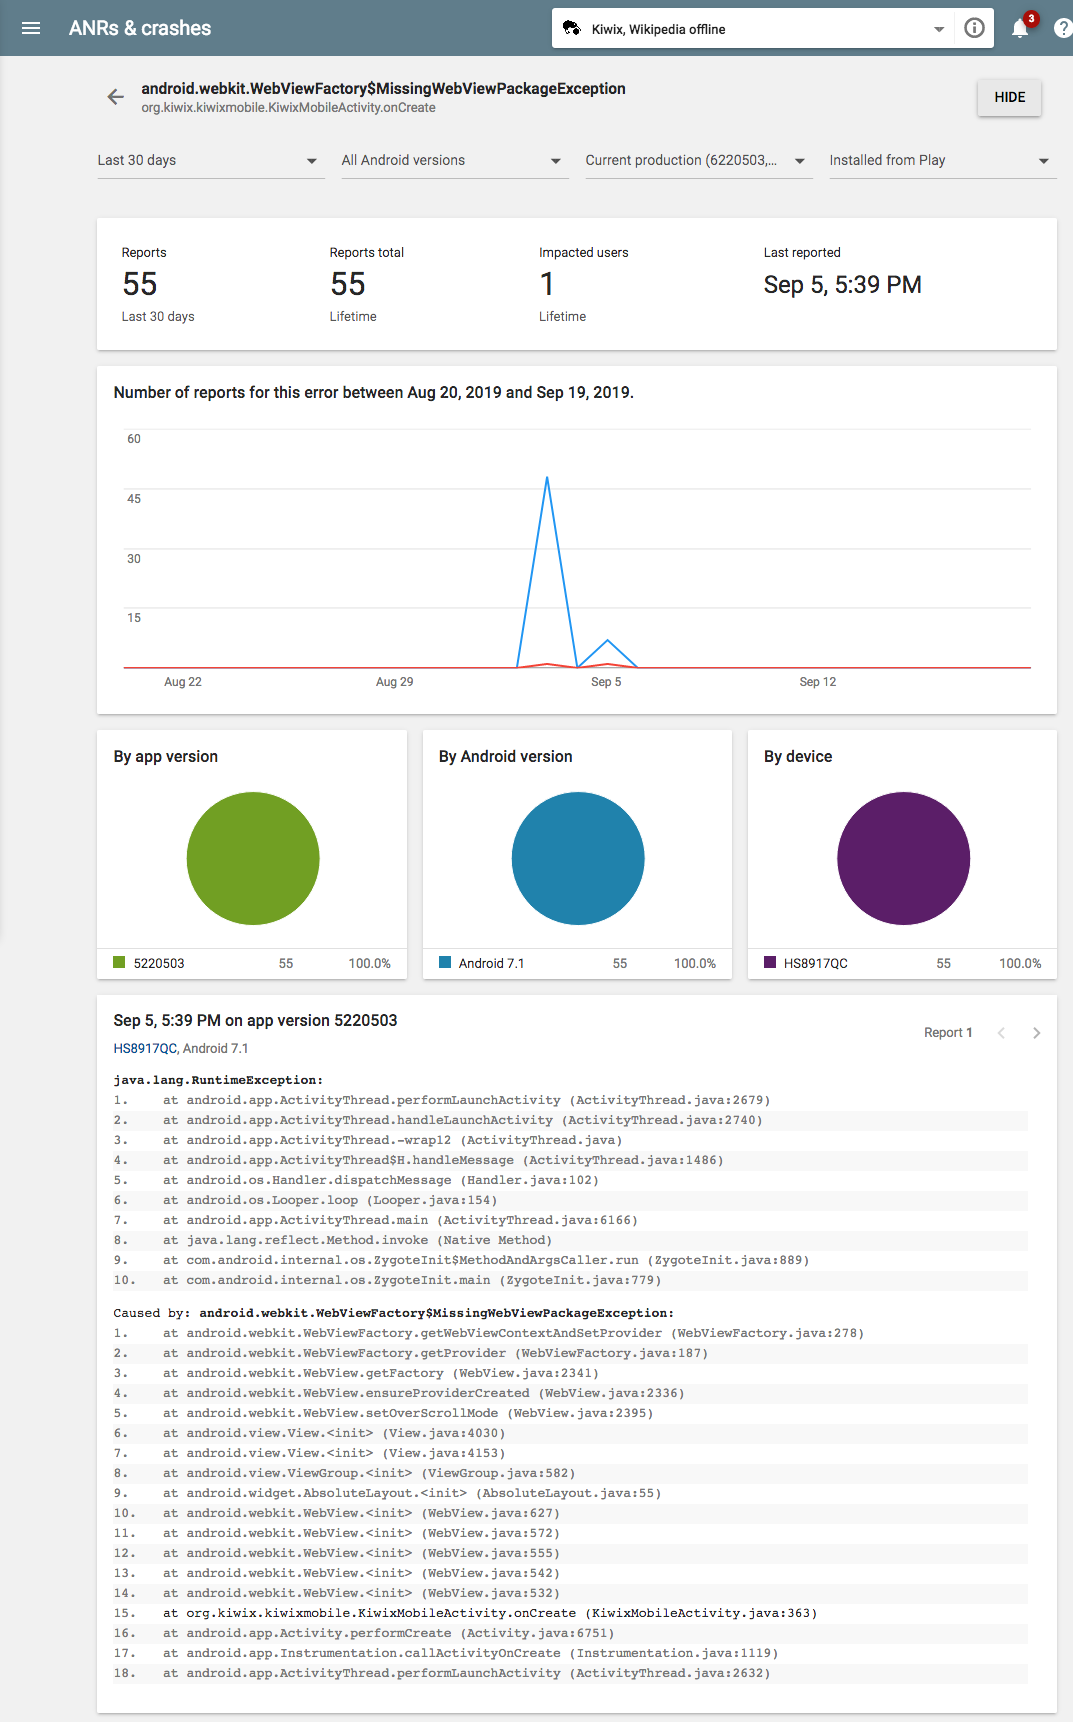
\includegraphics[width=\linewidth]{images/android-vitals-screenshots/55-crashes-WebViewFactory-MissingWebViewPackageException_2019-09-19-kiwix_trimmed.png}
    \caption{Kiwix Android 55 crashes for one user}
    \label{fig:55-crashes-WebViewFactory-MissingWebViewPackageException}
\end{figure*}

\FloatBarrier

\section{Macro topics}~\label{aata-macro-topics}
\julian{13-Jun-2022 This topic may move elsewhere, either partly or completely. If so, the effects on the artefacts (would still belong here). TBD when I've revisited that chapter.}

Macro-topics touch on multiple aspects of developing mobile apps. This research identified the following groupings of macro-topics:

\begin{itemize}
    \item Three of these have a common trait of \textbf{tradeoffs}\index{Tradeoffs} developers face, in ethics, in the use of third-party code, and in functionality.
    \item Two have a common trait of \textbf{scaling}\index{Scaling}: scaling use of mobile analytics by developers and within their engineering microcosm.
    \item Two cover the trustworthiness and fidelity of the mobile analytics as reflected in the artefacts.\emph{I have an inkling this material is better placed elsewhere in my thesis than this chapter. TBD.} 
\end{itemize}

\subsection{Tradeoffs}
At least three types of tradeoffs were evident in the artefacts: 1) the effects of ethical decisions by the project team (covered in \secref{aiu-ethics-and-pii-topics}, 2) downgrading functionality to obtain reliability, and 3) use of third-party vs locally developed functionality.

\section{Discussion}

\subsection{Fieldstones}
Explain how the absolute percentage of reliability scores is not necessarily a true reflection of the reliability of the app as the score is dependent on several factors including:

\begin{itemize}
    \item The settings on the device or in an app that gate whether analytics is provided to the mothership.
    \item The connectivity and transfer mechanism.
    \item Whether the ephemeral data is preserved on-device sufficiently to transfer it.
    \item Any filtering performed during transmission and/or reception of the data.
    \item Any filtering in the reporting.
    \item When and where the failure occurred.
    \item The date and time on the device (and perhaps on intermediate equipment).
    \item Whether the failure conditions occur.
\end{itemize}

Somewhere I need to present the improvements in the measured stability/reliability of the apps.